\documentclass[]{article}

\usepackage{hyperref}
\usepackage[parfill]{parskip}
\usepackage{titling}
\usepackage[a4paper, margin=1in]{geometry}
\usepackage{graphicx}
\usepackage[T1]{fontenc}
\usepackage{amssymb}
\usepackage{tabu}
\usepackage{float}
\usepackage{wrapfig}
\usepackage[svgnames]{xcolor}
\usepackage{colortbl}
\usepackage{multicol}

\pretitle{%
	\begin{center}
    	\vspace{-2cm}
		\LARGE
		
\includegraphics[width=6cm]{CSS-block}\\[\bigskipamount]
}
\posttitle{\end{center}}

\renewcommand{\familydefault}{\sfdefault}

%opening
\title{University of Bristol Computer Science Society \\ Sponsorship Packages 2016-17}
\author{}
\date{}

\begin{document}

\maketitle

\vspace{-1cm}

Welcome!

We are CSS, and we represent every Computer Science student at the University of Bristol. 

We organise social events; connect students with opportunities in industry and tackle the issues faced by our members. We serve hundreds of students, with a diverse range of interests and future career paths, and we'd love to connect you with them! 

\section*{Why sponsor us?}

\begin{center}
  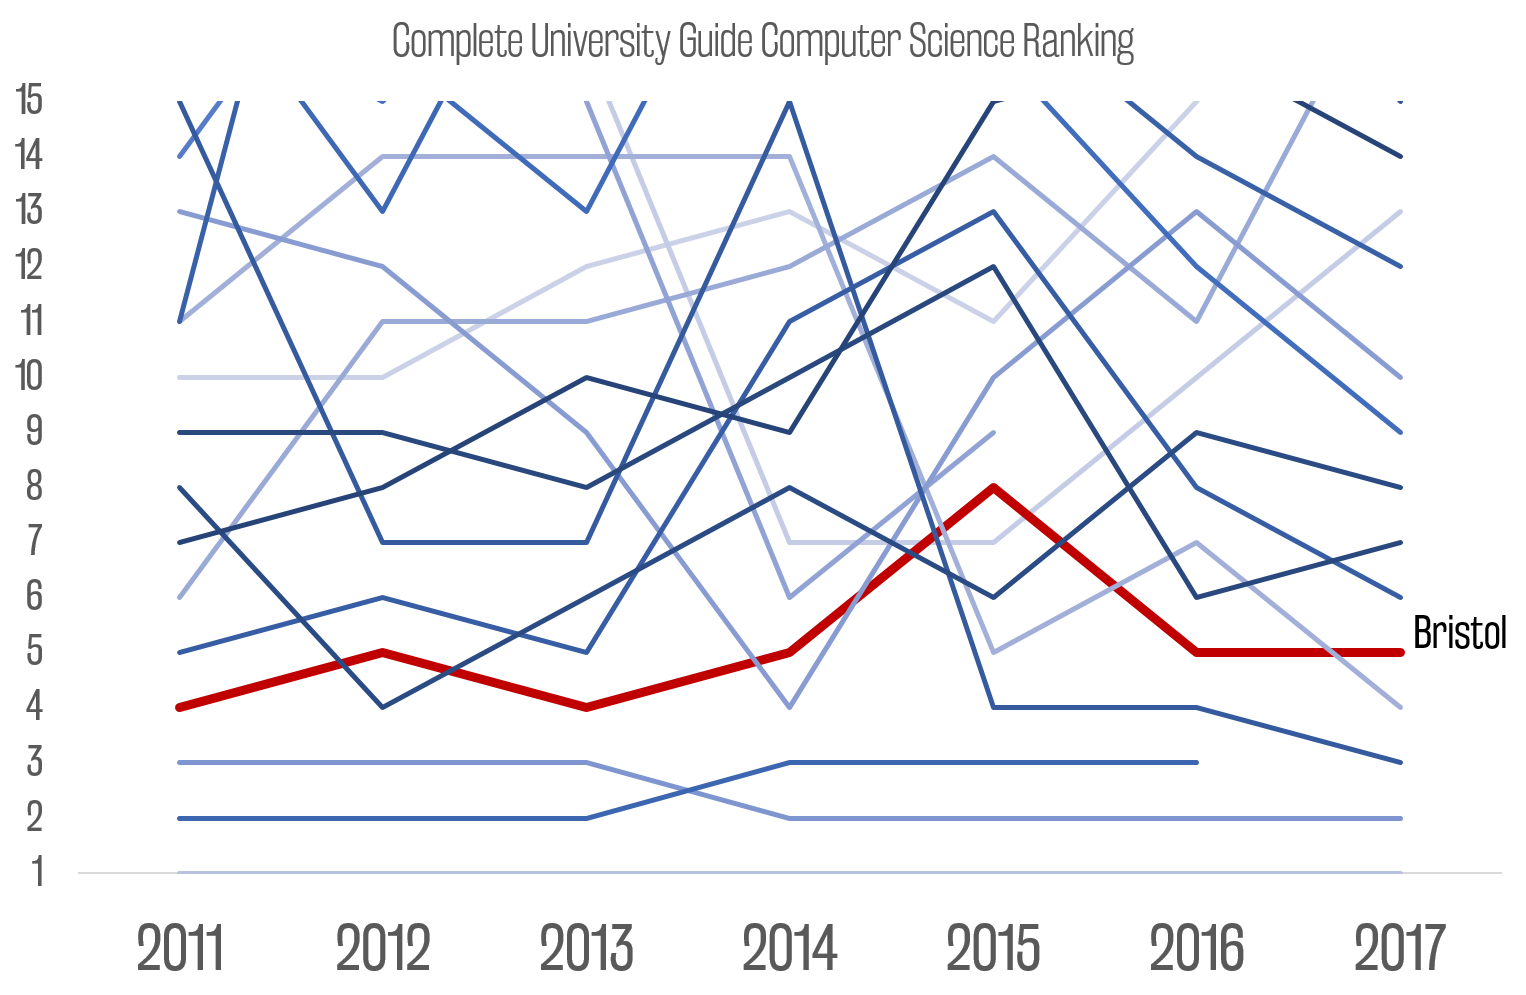
\includegraphics[width=0.4\textwidth]{ranking-chart}
  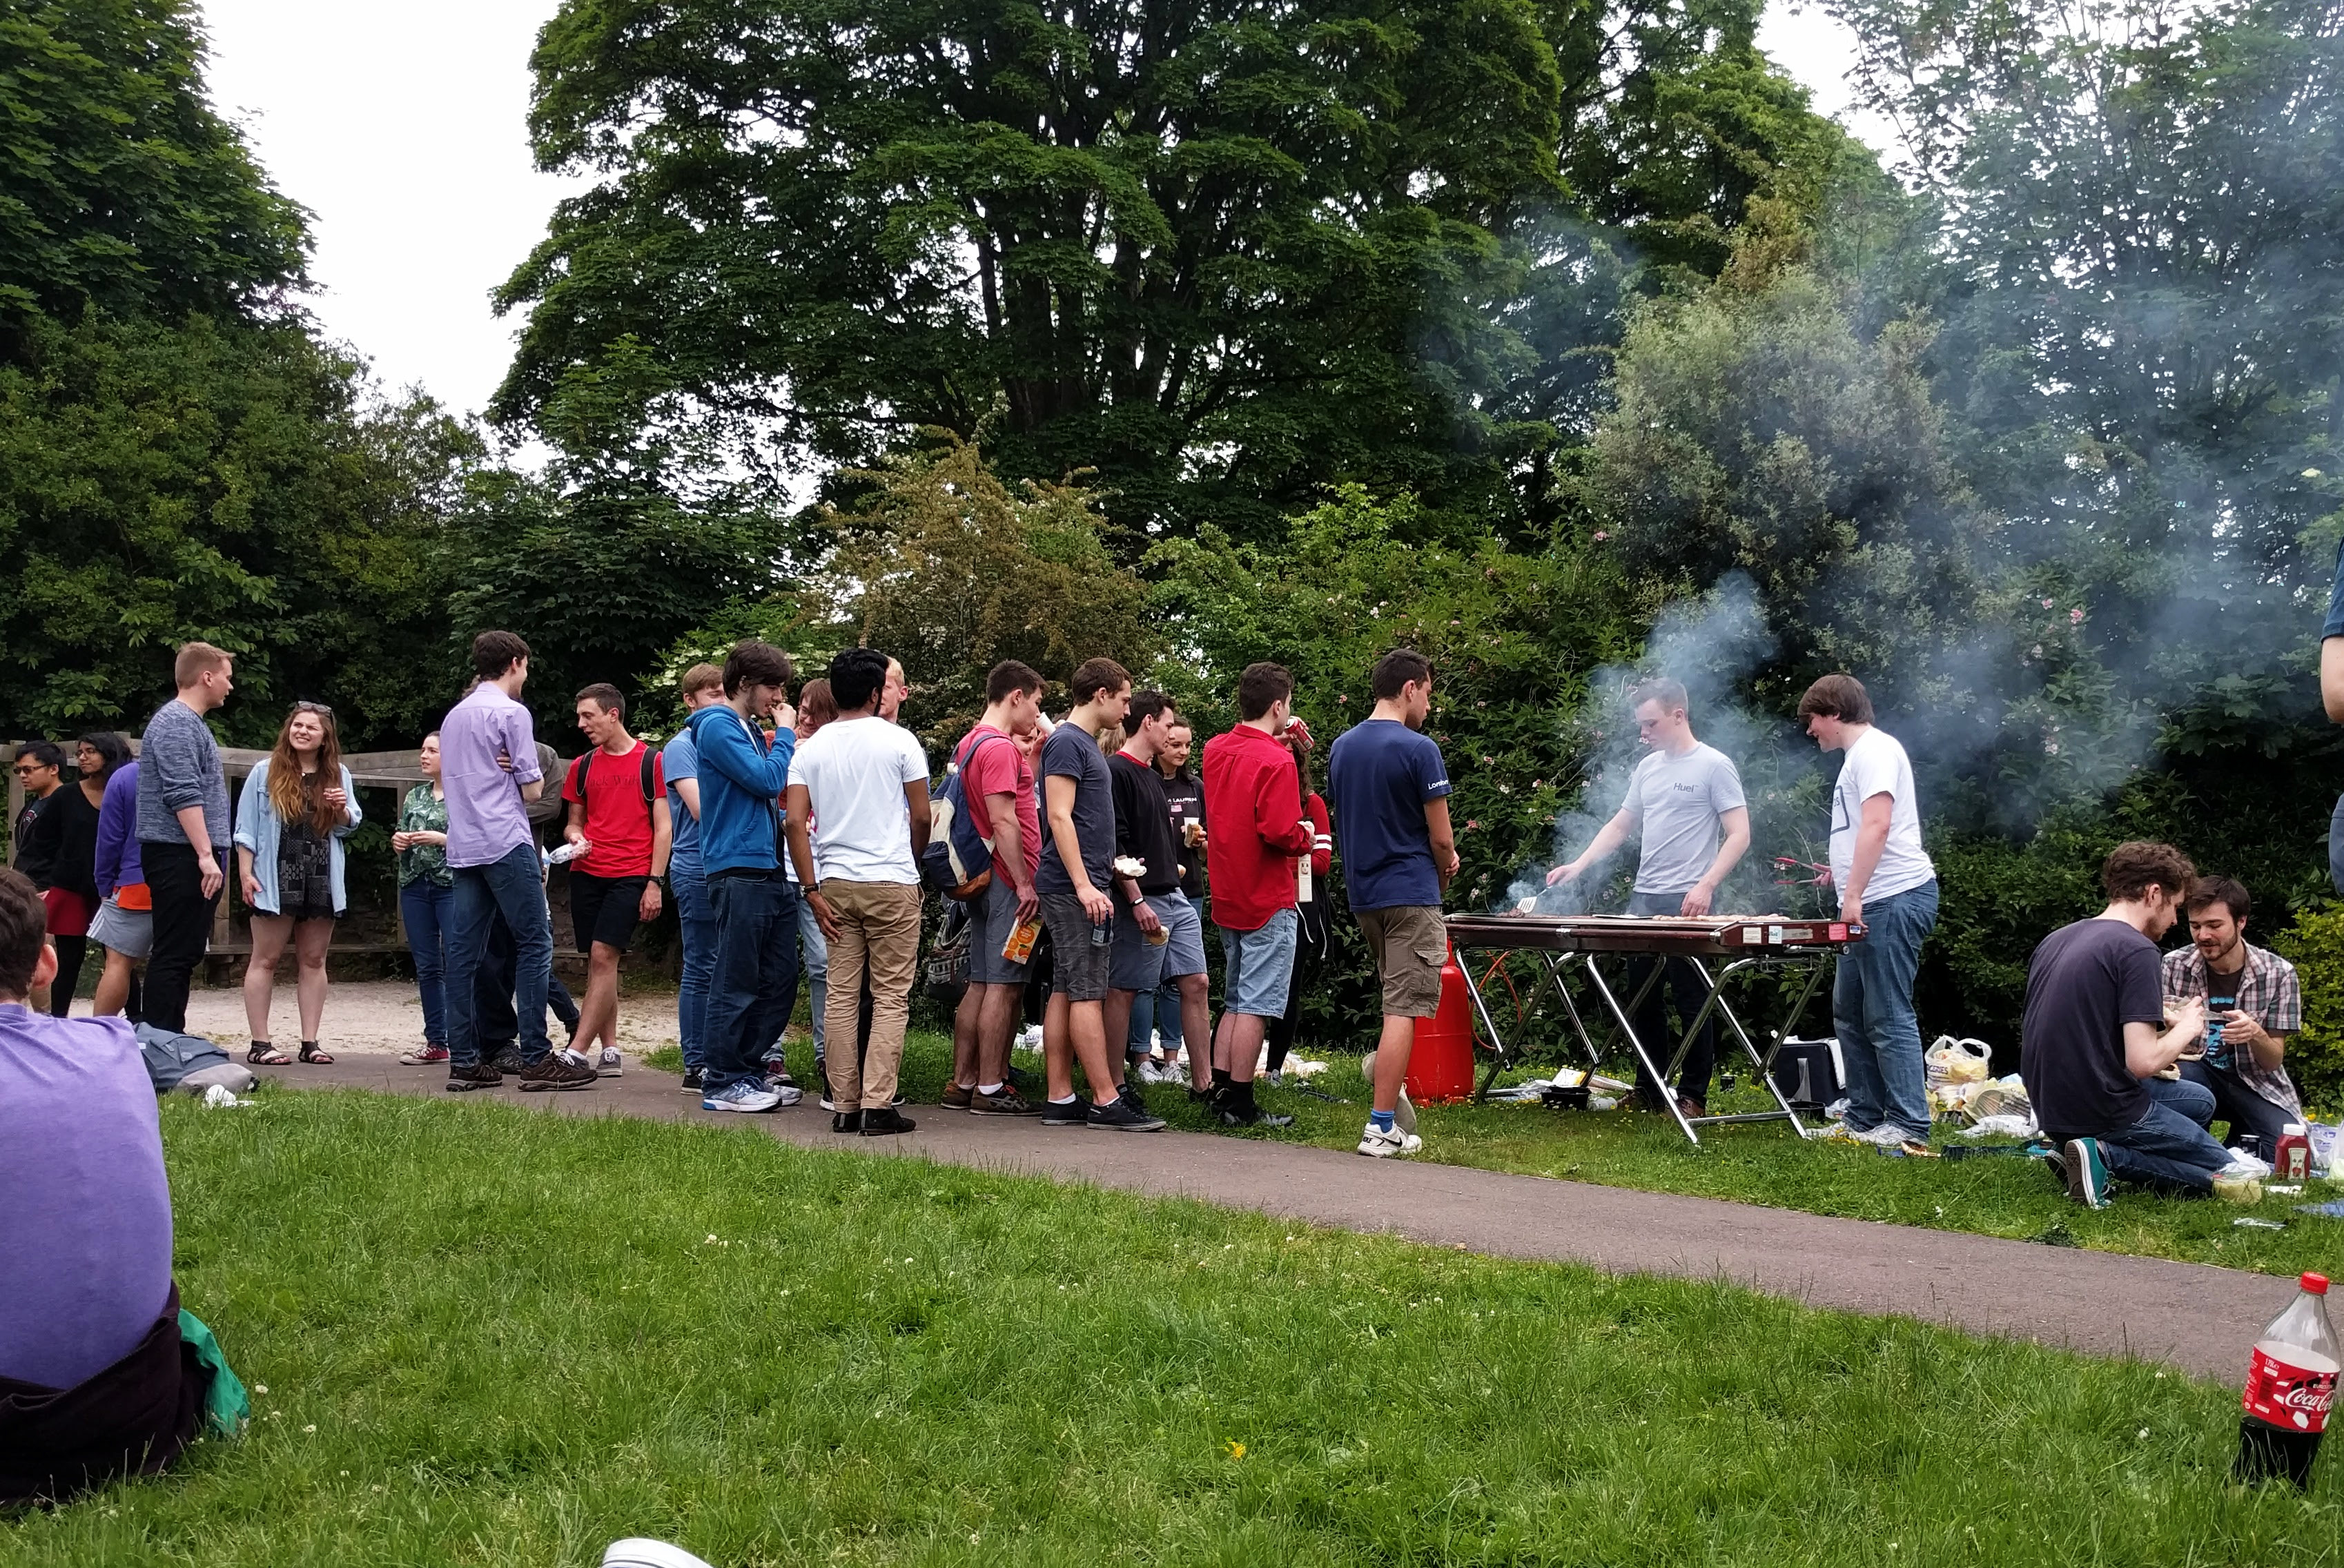
\includegraphics[width=0.4\textwidth]{bbq}
\end{center}

\begin{multicols}{2}
  \begin{itemize}
      \item Our department is consistently considered to be \textbf{in the top five Computer Science departments} in the UK.
      \item \textbf{Everyone studying Computer Science at the University of Bristol is automatically a member of CSS.} We have over 500 undergraduates, as well as more than 200 postgraduates, making us one of the largest societies at the University.
      \item \textbf{We run a number of popular events each year}: hackathons, discussion panels, talks, social events and more. These are a perfect opportunity for you to raise your profile among our students.
      \item We \textbf{work with other societies} in the University, including:
              \begin{itemize}
                  \item The University of Bristol Engineering Society (TUBES)
                  \item Bristol Electrical and Electronic Engineering Society (BEEES)
                  \item Women In Engineering
                  \item LGBT+ Engineers
              \end{itemize}
      \item We are in \textbf{constant communication with our members}, through our:
              \begin{itemize}
                  \item Facebook group (1300+ members including many alumni)
                  \item Website \footnote{\url{http://cssbristol.co.uk/}} (recently relaunched)
                  \item Twitter account (220 followers) \footnote{\url{https://twitter.com/cssbristol}}
                  \item Regular email newsletter (commencing September)
                  \item Physical noticeboard in the department (commencing September)
              \end{itemize}
           We can help you promote your message through all of these channels, as well as branding our major events and society t-shirts.
  \end{itemize}

\end{multicols}

\pagebreak

\section*{What options are available?}

We have a number of sponsorship options available. 

\subsection*{Sponsor us for a year}

We recommend investing in a year-long sponsorship of CSS. We have several suggested sponsorship tiers, but don't hesitate to ask us if you're looking for something specific!

\def\arraystretch{1.5}

\newcolumntype{b}{>{\columncolor{Sienna}}c}

\begin{tabu} to \textwidth { |X[3,l]|X[1,c]|X[1,c]|X[1,c]| }
	\hline
    										& Bronze & Silver & \textbf{Gold} \\
                                            & \pounds 899   & \pounds 1199  & \textbf{\pounds 1499} \\
    \hline
    \multicolumn{4}{|l|}{\textbf{Raise your profile among our students}} \\
    \hline
    Logo on our website						& \checkmark & \checkmark & \checkmark \\
    Logo on our hoodies						& 			 & \checkmark & \checkmark \\
    Logo on our t-shirts					&            & \checkmark & \checkmark \\
    \hline
    \multicolumn{4}{|l|}{\textbf{Meet students at the project fair}} \\
    \hline
    Invitation to fair     					&            & \checkmark & \checkmark \\
    Your own stand		  					&            &            & \checkmark \\
    \hline
    \multicolumn{4}{|l|}{\textbf{Get involved in events}} \\
    \hline
    Host your own event  					&            &            & \checkmark \\
    \hline
    \multicolumn{4}{|l|}{\textbf{Tech talks}} \\
    \hline
    Prioritisation over non-sponsors		& \checkmark & \checkmark & \checkmark \\
    Included catered talk					&            & 1		  & 1 \\
    \hline
    \multicolumn{4}{|l|}{\textbf{Communicate with our members}} \\
    \hline
    Profile on our website             		& \checkmark & \checkmark & \checkmark \\
    Promote jobs through our website 		& \checkmark & \checkmark & \checkmark \\
    Promote events through our website		& 			 & \checkmark & \checkmark \\
    Advertise in our email newsletter		&            & \checkmark & \checkmark \\
    Put up posters in the faculty           & 2x         & 4x         & Monthly \\
    Post on the society notice board        &            & 4x         & Dedicated space \\
    Dedicated email to all society members  &            &            & Each term \\
    \hline
\end{tabu}

All prices include VAT.

\pagebreak

\newgeometry{top=1.5cm,bottom=1cm}

\subsection*{Sponsor a single event}

Running an event allows you to talk directly to our students and show them:

\begin{itemize}
	\item Interesting technical problems you work on
    \item What it's like to work at your company
    \item What you're looking for in young engineers
\end{itemize}

Talks and other events are the perfect opportunity to find students who are already interested in your business.

\subsubsection*{Tech talk (\pounds 199 inc. VAT)}

Throughout the year, we invite engineers to talk about their experiences and technical work. You send the presenter; we organise food, drink, venue and advertising.

We usually expect an audience of around 40--50 people (variable depending on the availability and interest of students). 

\subsubsection*{Appathon}

Get involved with our major annual event: the 24-hour appathon.

\begin{itemize}
	\item Theme and name the event
    \item Your representatives on the judging panel
    \item Connect with promising programmers
    \item Leading up to the event, run talks/advice sessions for participants
\end{itemize}

\subsubsection*{Hackathon}

Host or assist a day long Hackathon.

\begin{itemize}
	\item Theme and name the event
    \item Get your hardware or software directly into the hands of students
    \item Run a talk introducing your company
\end{itemize}

\subsubsection*{CodeLounge}

\textbf{Our new event launching this year!} CodeLounge is aimed at the many Computer Science students who haven't programmed before they start at university. 

\begin{itemize}
	\item Help host or design the event
    \item Make an impression on students at the very start of their software engineering career
    \item Introduce your company to our new students
\end{itemize}

\subsubsection*{Something else?}

We run discussion panels, social events and much more for our members. If you would like to partner on the production of any kind of event, get in touch!

\section*{How do I sponsor you?}

We'd love to hear from you.

The best way to get in touch is to email our society vice-president, Codrin Popa (\href{mailto:vice-president@cssbristol.co.uk}{vice-president@cssbristol.co.uk}). Alternatively, you can email our society president, Hakeem Kushoro (\href{mailto:president@cssbristol.co.uk}{president@cssbristol.co.uk}). Let us know which packages you are interested in, and any questions you might have.

\restoregeometry

\end{document}
